\clearpage
\subsection{File Structures} % (fold)
\label{sub:file_structures}

When thinking about using using files, the one aspect that you need to spend the most time on will be the organisation of the data in the file. You need to ensure that the data you save includes sufficient information that it can be read back into the program at a later stage. Some common strategies are to:

\begin{enumerate}
  \item Write fixed size data blocks where possible.
  \item Store meta data\footnote{Meta data is data about your data.}, such as the number or size of variable data blocks.
  \item Alternatively, mark the end of variable sized or numbered data blocks with a \emph{sentinel} values.
\end{enumerate}

\begin{figure}[h]
   \centering
   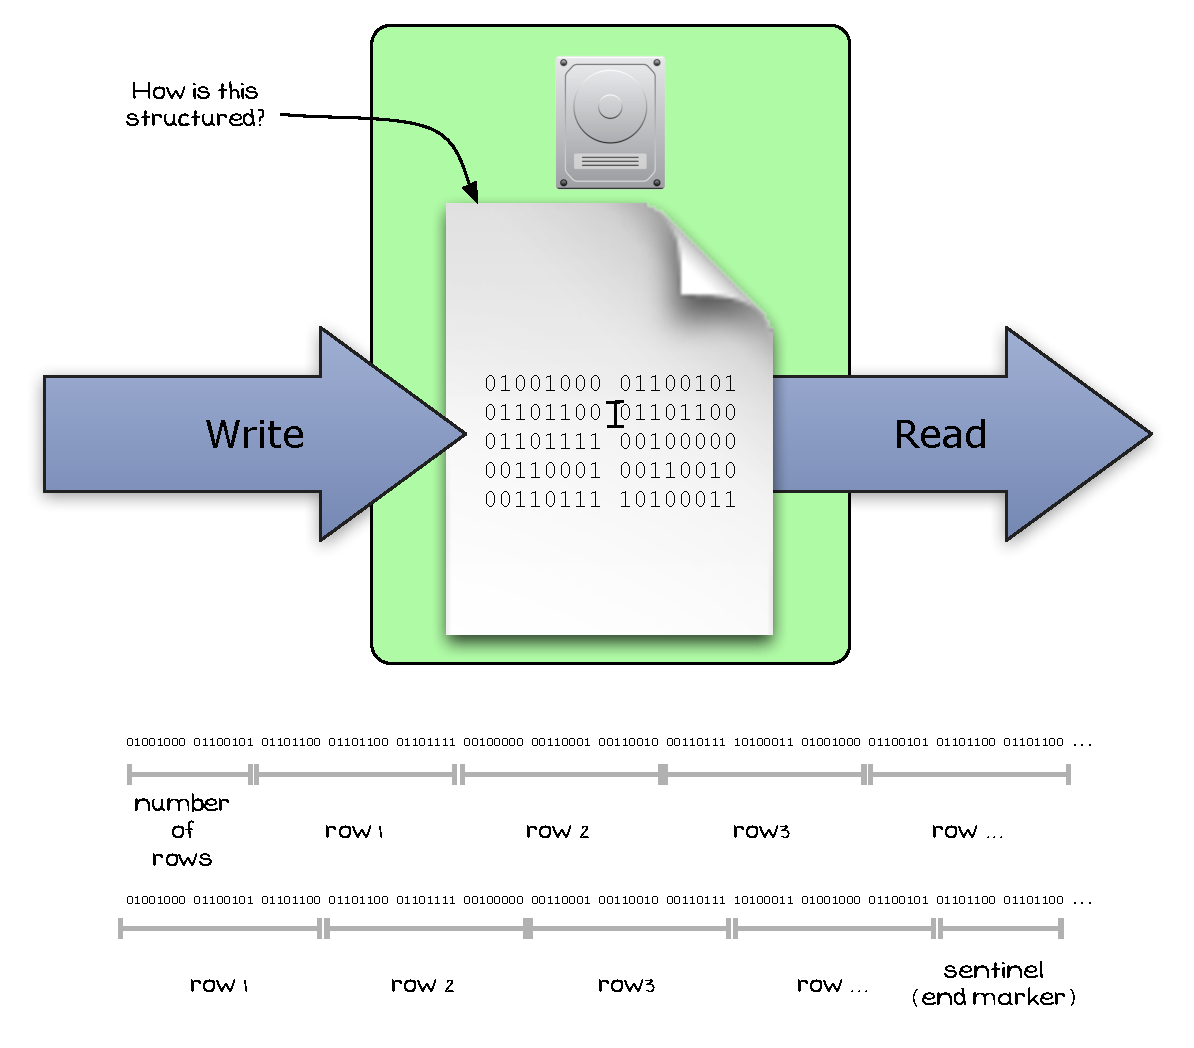
\includegraphics[width=0.9\textwidth]{./topics/file-io/diagrams/FileStructures} 
   \caption{You need to structure data within the file to make it possible to read back successfully.}
   \label{fig:file-structures}
\end{figure}

\mynote{
\begin{itemize}
  \item \fref{fig:file-structures} shows different ways of structuring a variable number of `row' values within a file.
  \item The row values are fixed size blocks, or use their own strategy to manage variable length data.
  \item One version stores the number of elements in the data before storing the data itself.
  \item An alternate strategy is to store a sentinel value at the end of the variable length data.\footnote{There is an end of file marker that can also be used for this purpose.}
\end{itemize}
}

% subsection file_structures (end)